\documentclass[a4paper,10pt]{paper}
\usepackage[margin=1.25in,footskip=0.25in]{geometry}

\usepackage[utf8]{inputenc}
\usepackage{natbib}
\usepackage{graphicx}
\usepackage{parskip}
\usepackage{amssymb}
\usepackage{rotating}
\usepackage{csvsimple}
\usepackage{hyperref}

\usepackage{adjustbox}
\usepackage{array}
\usepackage{booktabs}
\usepackage{multirow}

\newcolumntype{R}[2]{%
    >{\adjustbox{angle=#1,lap=\width-(#2)}\bgroup}%
    l%
    <{\egroup}%
}
\newcommand*\rot{\multicolumn{1}{R{90}{1em}}}% no optional argument here, please!


\usepackage{listings}
\usepackage{color}
\lstset{
   language=html,
   numbers=left,
   numberstyle=\tiny,
   breaklines=true,
   showstringspaces=false,
   basicstyle=\ttfamily,
   keywordstyle=\color[rgb]{0,0,1},
   commentstyle=\color[rgb]{0.133,0.545,0.133},
   stringstyle=\color[rgb]{0.627,0.126,0.941}
}

\graphicspath{ {./images/} }

%opening
\title{Designing a modular architecture for building web-based psychological experiments}
\subtitle{
Bachelor thesis, Cognitive Science \\
University Osnabrück, 2021}
\author{Marcel Klehr}

\begin{document}

\maketitle
\begin{abstract}
In the social and behavioral sciences, web-based experiments allow experimentors to recruit larger, more diverse subject pools with higher statistical power, and can speed up experiments dramatically, while being portable to any device with a browser. While web-based experiments have become increasingly popular, methods to construct them have been lacking in flexibility and simplicity. We introduce magpie, a modern, component-based, declarative JavaScript framework based on Vue.js for building web-based experiments of varying complexity with ease, including the possibility to have participants interact virtually.
\end{abstract}
\newpage 

\tableofcontents
\newpage 


\section{Introduction}
Web-based experiments are gaining more popularity in behavioural research, because of their flexibility and efficiency. From our analysis, we find that many existing tools for realizing such experiments lack sufficient flexibility and expressiveness. This lead to the creation of magpie, both a server for managing experiments and a client-side framework for implementing them.

Magpie experiments can be run directly on a local computer, and published online with ease. They can also be shared in an editable format and reused or adapted, enabling transparent replications and facilitating open science. Magpie is provided free of charge under an open-source license.

In this work, I initially examine prior work and competing software products with a set of requirements in mind. In the following section I explore the design goals and choices in relation to these requirements that lead to the implementation of magpie's client-side framework, its concepts, components, features and technical realization. Afterwards, I discuss limitations of the current design and future directions. Finally, I reach conclusions about the design and its applications.

In addition to this document, this thesis includes the creation of the full online documentation of magpie available at \url{https://magpie-manual.netlify.app} and \url{https://magpie-reference.netlify.app}.

\section{Web-based experiments}
Psychology and Social sciences have traditionally conducted research in close proximity to participants: in laboratory settings, after the fact in natural experiments or directly in the field. These modi have their limitations of capacity, speed, and subject diversity, especially when targetting a specific, possibly rare or remote population. The recent COVID-19 pandemic also severely inhibited direct-contact experiments due to contact-restricting preventative anti-infection measures.

Web-based experiments by contrast allow participants to take part in an experiment via the internet. This generally allows experimenters to recruit larger, more diverse subject pools, providing higher statistical power, and can speed up experiments dramatically due to their unsupervised nature.

As participants are usually unmonitored, however, experimental instructions may be ignored or read too carelessly, potentially leading to lower quality data. Researchers are additionally largely unable to control the environment, potentially inucrring significant distractions during the experiment. Technical details such as network connection speed and reliability, computer and browser types as well as screen resolution may contribute to additional variance in the data.

Although these uncontrollable factors suggest decreased reliability of web-based experiments, experiments on LabintheWild have been shown to replicate previous in-lab results. \citep{Gajos2015} In similar fashion, \citet{Schoeffler2013} compared results from laboratory and web-based studies and found no significant differences. \citet{RRMWSC2013} even concluded that unsupervised web-based experiments with large subject pools have benefits over smaller, supervised lab experiments, outweighing their potential costs with their larger sample size, such that patterns that were not significant in the lab were significant on the web.

\section{Requirements}
In our analysis of prior work as well as in the design of magpie, we focus on the following features we deem desirable.

An \textbf{Open Source} license is essential for common access to the tool in question as well as sustaining development. \textbf{Recruiting flexibility} requires that the tool in question does not restrict recruiting to a specific participant recruiting platform. Tools should offer a \textbf{Framework} for building custom experiments rather than a mere library to select experiments or trials from. \textbf{Implementation flexibility} indicates a Turing complete programming environment. \textbf{Sharable customizations} are important to facilitate re-use of custom experiment parts across experiments. \textbf{Interactivity} indicates the ability of a tool to allow participants to interact online during an experiment, both synchronously and asynchronously. \textbf{Dynamicity} indicates the ability to use a participant's past responses to control the course of the experiment. This is useful for applying Optimal Experiment Design that takes into account participant's responses in a variation of \citet{Ouyang2016}. \textbf{Multimedia support} indicates the possibility of including image, audio and video stimuli in experiments. A \textbf{Catalogue} of a wide variety of building blocks necessary for different experiment and task types.

\section{Analysis of prior work}
There are a variety of pre-existing software packages attempting to aid in the construction of web-based experiments. In the following we examine some prominent candidates.

\textbf{OpenSesame} \citep{Mathot2012} was mainly designed to be used for offline lab experiments in the fields of psychology, neuroscience and experimental economics. It is licensed under the open-source GNU General Public License and runs across various platforms utilizing Python.

Using an extension called OSWeb, experiments built with OpenSesame can be run in the browser, albeit with somewhat limited functionality. The fact that OpenSesame was designed to be run with Python naturally limits the range of features provided in the browser as not all functionality is ported to the browser. The main strength of OpenSesame, its graphical editor, is also its main weakness: Realizing more complex experiments is often non-trivial with a certain amount of programming knowledge still necessary (e.g. for validating form input, counterbalancing, custom layouts, programmatically generating loop tables) and the possibilities limited by OpenSesame's structure. While dynamic experiments are possible via code blocks, it doesn't offer interactivity between participants.

\textbf{PsyToolkit} \citep{Stoet2012} is an all-in-one solution for web-based experiments, offering study design, hosting and even data analysis. It appears mainly geared toward students who need a simple solution to run their experiments and implements a custom imperative scripting language for realizing experiments, which appears rather simplistic and doesn't allow for much experimental complexity or customization. It does not allow for interactivity or dynamicity.

\textbf{psiTurk} \citep{Gureckis2016} is mainly a server-side framework for integrating web-based experiments with Amazon Mechanical Turk and cannot by used with other recruiting platforms. It only aids minimally in developing the actual experiments and thus has to be combined with a different front-end framwork.

\textbf{jsPsych} \citep{Leeuw2015} in contrast offers a JavaScript interface to realize experiments, theoretically allowing implementers to take advantage of the power of the web platform. It interoperates with JATOS \citep{Lange2015} as a backend and offers a wide range of pre-built templates called "plugins" to be used for experiments. However, beyond the existing templates, implementing custom functionality and recombining different templates is non-trivial as there are no built-in components and no simple built-in framework for assembling custom trials. Interactivity and dynamicity are not offered.

\textbf{LIONESS-lab} \citep{Giamattei2020} is a full-featured solution for developing interactive experiments, offering a graphical experiment builder and automatic testing of experiments. While experiments can be equipped with more complex logic by virtue of JavaScript code, the project's scope and built-in building blocks focus largely on economic experiments and do not appear to be extensible. Runnable experiments are a combination of server-side management code and client-side code which requires technical setup effort and skills for each new experiment, making self-hosted deployment non-trivial. However, a free hosting service is available. LIONESS lab also offers interactivity and dynamicity.

Similar to LIONESS-Lab, \textbf{Labvanced} \citep{Scicovery2018} offers a full-featured graphical experiment editor, albeit with a much wider range of building blocks for various stimuli as well as interactivity. Labvanced is proprietary and relies on a subscription model.

\textbf{z-Tree} \citep{Fischbacher2010} is a popular framework for conducting economic experiments, written in C++ and is thus not web-based although it can be made to work via the internet. z-Tree allows for rather complex experimental setups, but its scope and components are focused on economic experiments.

\textbf{Dallinger} \citep{Suchow2016} is a server side experiment manager for automatically recruiting participants from Amazon Mechanical Turk, allowing to group them and facilitating information exchange in interactive experiments. Dallinger has a minimalistic client-side JavaScript API, requiring the use of third-party libraries for implementing rich web experiments. Experiments are modeled with a complex server-side framework that allows automating participant interactions for testing purposes, but requires sophisticated software engineering efforts to realize experiments.

\textbf{lab.js} \citep{Henninger2020} is a client-side framework featuring both an application programming interface and a graphical user interface  for building web-based experiments. It interoperates with JATOS \citep{Lange2015} as a backend. Although the graphical experiment builder simplifies usage greatly, lab.js only offers few basic built-in components and doesn't build upon existing JavaScript frameworks for simplicity and efficiency. It does not offer interactivity.

See Table \ref{tab:competition} for an overview and comparison with magpie. From my analysis, I find that many existing tools for realizing such experiments lack sufficient flexibility and expressiveness, providing only a limited set of components or commands that can be used, often without the ability to recombine them. Some do provide the ability to build custom components, but only with a steep learning curve, others offer a graphical editor to gain simplicity, while sacrificing flexibility.

\begin{table}[]
\begin{tabular}{lllllllllll}
                      & \rot{OpenSesame} & \rot{PsyToolkit} & \rot{psiTurk}    & \rot{jsPsych}    & \rot{LIONESS-lab} & \rot{Labvanced}  & \rot{zTree}      & \rot{Dallinger}  & \rot{lab.js}     & \rot{magpie}     \\
Web                        & \checkmark & \checkmark & \checkmark & \checkmark & \checkmark  & \checkmark &            & \checkmark & \checkmark & \checkmark \\
Free software              & \checkmark & \checkmark & \checkmark & \checkmark & \checkmark  &            & \checkmark & \checkmark & \checkmark & \checkmark \\
Reruiting flexibility      & \checkmark & \checkmark &            & \checkmark & \checkmark  & \checkmark &            &            &            & \checkmark \\
Sharable customizations    &            &            &            & \checkmark &             & ?          & ?          &            & \checkmark & \checkmark \\
Framework                  & \checkmark & \checkmark &            &            & \checkmark  & \checkmark & \checkmark &            & \checkmark & \checkmark \\
Catalogue                  & \checkmark & \checkmark &            & \checkmark & \checkmark  & \checkmark & \checkmark &            &            & \checkmark \\
Interactivity              &            &            &            &            & \checkmark  & \checkmark & \checkmark & \checkmark &            & \checkmark \\
Dynamicity                 & \checkmark &            &            &            & \checkmark  & ?          & ?          & ?          & ?          & \checkmark \\
Multimedia                 & \checkmark & \checkmark          &            & \checkmark & \checkmark  & \checkmark & ?          &            &            & \checkmark \\
Implementation flexibility & \checkmark & \checkmark &            & \checkmark & \checkmark  & \checkmark &            &            & \checkmark & \checkmark
\end{tabular}
\caption{Overview of features}
\label{tab:competition}
\end{table}

\section{Design}

\subsection{Design goals and choices}
A main goal of designing magpie was to provide implementers with a conceptually simple framework for building experiments that should be employable as a tool for teaching the basics of experimental design. At the same time the framework should be general and expressive enough to facilitate building complex interactive experiments without major software engineering skills.

A key concept for bridging this divide is modularity and composability: Offering a catalogue of building blocks in varying granularity to ease assembly of simple experiments with larger, more rigid components, but also allowing intricate customization via smaller, flexible components that integrate with each other.

To this end, taking advantage of a modern, reactive and component-based JavaScript framework like Vue.js \citep{You2014} allows for fast progress and interoperability with a large catalogue of open source modules already built on that same framework, while avoiding mistakes that others have already made and corrected. Choosing a reactive framework is a major benefit for implementation effiency, because the view layer updates automatically based on the provided data, reducing the amount of code to write.

A graphical editor is explicitly not part of the scope of this project at the moment. The emphasis on free customizability necessitates the use of a programming language rather than the limited freedom of a graphical editor. However, building a graphical editor on top of magpie is still possible in future work.

Another goal was easy interoperability with participant recruiting platforms such as Amazon Mechanical Turk and Prolific.

\subsection{Overview}
Magpie consists of two parts that each have their own responsibilities: a server-side service and a client-side framework. These two parts, although integrating with each other, are largely independent. The server handles experiment management, configuration and data storage. It is designed to be the backend for multiple different experiments that are possibly hosted elsewhere.

The client-side framework builds upon Vue.js, a reactive JavaScript framework, to allow the assembly of experiments as single-page web applications that connect to the backend server to store results and exchange information with other participants for interactive experiments. The client-side framework acts both as a component library providing building blocks for experiments as well as an API to the backend server and other utility functions.

From my analysis, I find that many existing tools for realizing web-based experiments lack sufficient flexibility and expressiveness. In the spectrum between usability and flexibility, I believe magpie's client-side to be a worthwhile compromise: Utilizing the expressiveness and simplicity of Vue.js \citep{You2014}, which is a declarative and reactive component framework for the web, magpie provides a large catalogue of components that can be recombined and customized to build experiments of any complexity. This makes simple experiments barely harder to implement than writing normal HTML, while scaling to the complexity of, for example, a fully interactive behavioral economics experiment.

\subsubsection{Conceptual Framework}

\begin{figure}[h]
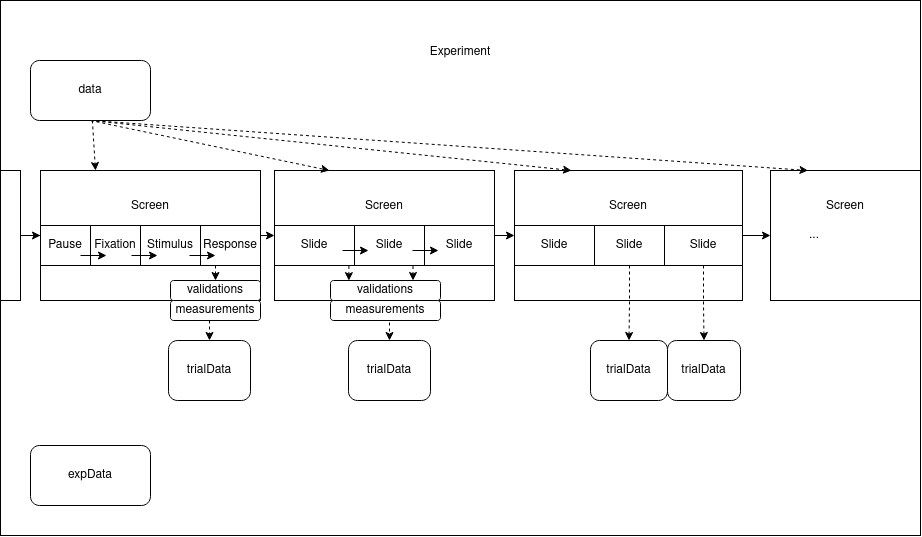
\includegraphics[width=\textwidth]{experiments_schema.png}
\caption{Conceptual schema of a magpie experiment}
\label{fig:concepts}
\end{figure}

A magpie experiment (see Figure \ref{fig:concepts}) firstly consists of the data used to build the experiment, also known as independent variables.
This could be textual, visual or auditory stimuli that are presented to the participants or possible choices that the participants can make.

Every experiment is further composed of a series of screens that participants go through sequentially. Such a screen could display instructions on how to participate, or present an actual trial task to the participant. Usually one trial will be realized per screen. This is similar to what researchers are used to from OpenSesame \citep{Mathot2012} and a natural representation of many experiment paradigms.

A screen consists of a sequence of one or more slides. Slides simplify dynamic presentation of more intricate tasks. They are also displayed sequentially, giving experimenters the opportunity to display fixation points, or enforce pauses between stimulus and response. This design was chosen in inspiration from the design of computer-based psychological studies such as \cite{Todd2004}. A slide can contain arbirtray components from stimulus-presenting components, over interactive chat components, to response-recording components like a rating scale.

Anytime during a screen, result data rows can be saved directly which will be sent to the magpie server when the experiment is completed. To make collecting measurements across slides easier, data can also be gradually accumulated in a per-screen `measurements` object. This allows validating the data and saving all data in one go, once a trial is completed.

\subsection{Components}
Magpie provides basic stimulus components like playing audio files, video files, displaying image files, text, a self-paced reading component, a tone Synthesizer and a canvas for displaying dynamic visual stimuli. Responses can be recorded using dropdown inputs, a forced choice input, a single and a matrix multiple choice input, a slider input, a rating scale, a free text box, a key press input, a constant sum range slider, an image selection input, a text completion input and a rank order input.

These finer grained components offer essential features that can be recombined in a variety of ways to form trials of any complexity.
To ease the realization of experiments, there are many pre-built screen components available for usage, allowing the quick assembly of simple experiments out of coarse building blocks, utilizing the above fine graned building blocks under the hood. These trial screens follow a life cycle of five slides: pause, fixation, stimulus presentation, response collection and feedback. All phases except response collection are optional, and all phases can be configured with a timeout or a manual trigger to go to the next phase. Additionally, implementers can add a Question under Discussion text, a question and a slot for each of the four life cycle phases, that can be filled with custom content, for ease of use.

All screen components allow setting a screen title and a progress percentage which will be displayed in a progress bar.

In addition to normal response inputs, magpie also features eye and mouse tracking in order to measure the participants' thought process in more detail.

\subsection{Dynamic experiments}
Iterated experiments allow using data from past participants in later trials for new participants. This allows the creation of, for example, iterated narration experiments (similar to the game of telephone).
Magpie requires three basic settings on the server for running an iterated experiment: The number of variants, which defines how many different experimental settings there will be; the number of chains, which defines how many closed participant groups there will be; and the number of generations, which defines how many participants are in one chain.

\subsection{Interactive experiments}
Interactive experiments allow participants to interact with each other in some form, for example as rational decision-makers with strategic interactions in a mathematical model, as is frequently described in Game theory. On the client-side, magpie provides components for structuring interactive experiments, such as a screen to wait until the required number of participants in the group are online. To allow the flexible realization of any kind of interactivity, magpie allows sending and listening to events between individual participant sessions. Additionally, it keeps track of which participants currently see the same screen and assigns pseudonymous names and colors to all participants that can be used in experiments for easier identification during interaction.

\subsection{Technical realization}
Technologically, the client-side framework is based on Vue.js \citep{You2014}, an open-source front-end JavaScript framework for building web-based user interfaces and single-page applications. It facilitates declarative, reactive rendering and component composition, which is in contrast to traditional imperative programming, and greatly eases reasoning about and implementation of applications. Declarative rendering is facilitated by allowing to extend normal HTML code with behavior-invoking directives and stateful custom elements.

Magpie experiments are compiled using Vue.js's standard tooling, which provides an auto-reloading development server as well as static builds that can be deployed anywhere on the internet.

\subsubsection{Example 1: Mental rotation experiment}
The following example shows the code for a simple mental rotation experiment. The initial screen would display instructions to the participant, but is excluded here for brevity. Afterwards, the code iterates over a list of trial objects, defined elsewhere and constructs a new KeypressScreen for each. KeypressScreen is a built-in screen with four life cycle phases: Two seconds pause and one second fixation, as defined in the screen's properties. Third and fourth phase are merged together, by default, where the third phase displays the contents of the \texttt{\#stimulus} slot and the fourth phase allows responding using the F or the J key on the keyboard, which will indicate whether the participant thinks the two models in the picture are the same or different. The screen automatically records response time and response. (Find more information on built-in screens can be found at \url{https://magpie-manual.netlify.app/01_designing_experiments/00_built-in_screens/})

After the trial screens are completed the code shows a post-test screen, which asks the participants for demographic information. Finally the last screen will submit the data to the server and thank the participant when everything is completed.

\begin{lstlisting}[language=html]
<Experiment
  title="Mental rotation task"
>
    <template v-for="(task, i) of trials">
      <KeypressScreen
        :key="i"
        :progress="i / trials.length"
        :pauseTime="2000"
        :fixationTime="1000"
        :keys="{ f: 'different', j: 'same' }">
        <template #stimulus>
          <img :src="task.picture" />
        </Slide>
        
      </KeypressScreen>
    </template>

    <PostTestScreen />

    <SubmitResultsScreen />
</Experiment>
\end{lstlisting}


\subsubsection{Example 2: Simon Task}
The following example shows the code for a Simon Task experiment. The code in this example leaves out the instructions to the participants. The code iterates over a list of trial objects, defined elsewhere and constructs a new KeypressScreen for each.

The screen will first display fixation cross for a random duration between 1200ms and 2700ms, specified by the \texttt{fixation-time} attribute. Afterwards the simulus is displayed allowing a response with the Q and P keys. The response is stored in \texttt{\$magpie.measurements.response}. The stimuli are displayed using the built-in canvas components, displaying the square or circle left or right of the screen. The Record component adds the trial data to the result measurements. The \texttt{response-time} attribute sets a timeout of three seconds to respond, after which the participant is shown the feedback screen which tells them to respond more quickly if they haven't responded yet.

After the trial screens are completed the code shows a post-test screen, which asks the participants for demographic information. Finally the last screen will submit the data to the server and thank the participant when everything is completed.

\begin{lstlisting}[language=html]
<Experiment title="Simon task">

    <template v-for="(task, i) of trials">
      <KeypressScreen :key="i"
          :keys="{q: 'circle', p: 'square'}"
          :fixation-time="Math.floor(Math.random() * (1500) + 1200)"
          :response-time="3000">
        <template #stimulus>
          <CanvasStage
              :config="{width: 800, height: 100}">
            <CanvasLayer>
              <CanvasCircle
                  v-if="task.target_object === 'circle"
                  :config="{
                      fill: 'lightblue',
                      radius: 50,
                      x: task.target_position === 'left' ? 50 : 700,
                      y:50
                  }"
              />
              <CanvasRect
                  v-if="task.target_object === 'square'"
                  :config="{
                      fill: 'lightblue',
                      width: 100,
                      height: 100,
                      x: task.target_position === 'left'? 50 : 700,
                      y:0
                  }"
              />
            </CanvasLayer>
          </CanvasStage>
          <Record :data="{
            ...task
          }" />
        </template>

        <template #feedback>
          <p v-if="!$magpie.measurements.response">
          	Please answer more quickly
          </p>
          <Wait v-else :time="0" @done="$magpie.nextScreen()" />
        </Slide>
      </Screen>
    </template>

    <PostTestScreen />

    <SubmitResultsScreen />
</Experiment>
\end{lstlisting}

\subsubsection{Example 3: Public goods experiment (interactive)}
The following example shows the code for a public goods experiment, an interactive paradigm from behavioral economics. The code in this example leaves out the instructions to the participants. Before the trials start, the ConnectInteractiveScreen makes sure the socket connection to the server is active and the necessary number of participants have joined the experiment. The code then iterates ten times, and constructs a new raw Screen for each iteration.

The first slide of the screen will wait for all participants to view the same screen and reset local variables tracking the state of the trial. Once all participants are viewing the same screen, the second slide lets each of them select an amount of their stash to donate to the group using a slider input. When they submit their selection, \texttt{submitDonation} is called, which broadcasts the selected value to all participants of this session (s. line 113). The next slide waits for donations from all other participants to have come in, which are recorded by the socket listener in line 88 and checked in line 96 as a computed variable.

Once all participants have donated an amount, the last slide displays the reward they have received as well as their new balance. When the participant clicks on the displayed button, the results are saved and the next screen will be displayed (s. line 61), which is either another trial, or the post test screen.

After the trial screens are completed the code shows a post-test screen, which asks the participants for demographic information. Finally the last screen will submit the data to the server and thank the participant when everything is completed.

\begin{lstlisting}[language=html]
<template>
  <Experiment title="Public Goods Experiment">
  
    <ConnectInteractiveScreen />
    
    <template v-for="i of 10">
      <Screen :key="i">
        <Slide>
          <WaitForParticipants
            @done="
              resetPool();
              $magpie.nextSlide();
            "
          />
          <p>Waiting for participants...</p>
        </Slide>

        <Slide>
          <p>Your balance is {{ test_stash }} tokens.</p>
          <p>Please select an amount to donate.</p>
          <SliderInput
            :tooltip="true"
            :max="test_stash"
            :response.sync="$magpie.measurements.amount"
            left="0"
            :right="test_stash + ''"
          />
          <template v-if="typeof $magpie.measurements.amount !== 'undefined'">
            <p>
              You are donating {{ measurements.amount }} tokens to the group.
            </p>
            <button
              @click="
                submitDonation($magpie.measurements.amount);
                $magpie.nextSlide();
              "
            >
              Go
            </button>
          </template>
        </Slide>

        <Slide>
          <p>Please wait for all participants to make their move.</p>
          <Wait
            v-if="allParticipantsDonated"
            :time="0"
            @done="$magpie.nextSlide()"
          />
        </Slide>

        <Slide>
          <p>
            You have donated {{ $magpie.measurements.amount }} tokens and
            received {{ reward }} tokens.
          </p>
          <p>Your new balance is {{ new_stash }}</p>
          <Record :data="{ reward }" />
          <button
            @click="
              $magpie.saveAndNextScreen();
              updateStash();
            "
          >
            Next round
          </button>
        </Slide>
      </Screen>
    </template>

    <PostTestScreen />

    <SubmitResultsScreen />
  </Experiment>
</template>

<script>
export default {
  name: 'App',
  data() {
    return {
      pool: 0,
      donated: 0,
      test_stash: 100,
      amount: 0
    };
  },
  socket: {
    donate(amount) {
      this.amount = amount;
      this.pool += amount;
      this.donated++;
    }
  },
  computed: {
    allParticipantsDonated() {
      return this.donated === this.$magpie.socket.active.length;
    },
    reward() {
      return (this.pool * 1.3) / this.donated;
    },
    new_stash() {
      return this.test_stash - this.amount + this.reward;
    }
  },
  methods: {
    resetPool() {
      this.pool = 0;
      this.donated = 0;
      this.amount = 0;
    },
    submitDonation(amount) {
      this.$magpie.socket.broadcast('donate', amount);
    },
    updateStash() {
      this.test_stash = this.new_stash;
    }
  }
};
</script>

\end{lstlisting}

\section{Limitations and future directions}
A limitation of using Vue.js is the required build step for publishing experiments. Thus, making changes to existing experiments is only possible when the required toolchain is installed. This is a trade-off towards the usability of the live-reloading and modularity features of modern JavaScript frameworks. Magpie also still lacks built-in screens for a range of trial types, such as random dot kinematograms or visual search tasks. A key limitation is the need to write code in order to build experiments with magpie, a trade-off we find worthwhile to allow implementers greater flexibility. However, this does not exclude the possibility of building a graphical editor in the future.

Future work on magpie should include measures to improve reliability of experiments, such as "virtual chinrests" \citep{Li2020}, other types of visual display size calibration, the possibility of excluding participants based on the inavailability or inadequacy of certain browser features and recording distractions such as leaving the active browser tab.

Another avenue for improvement is interoperability with JATOS \citep{Lange2015} and Sona \citep{SonaSystems2002}.
\section{Conclusion}
Web-based scientific experiments offer higher statistical power at a lower cost and effort with only marginal disadvantages. Magpie's client-side leverages the advantages of modern JavaScript frameworks to offer a simple yet powerful framework for building such experiments. Its conceptual structure facilitates realizing basic as well as complex and even interactive experimental paradigms, while striking a balance between usability and expressiveness. Provided under an open source license, magpie facilitates open science, and eases the replication process. Fully relying on the power of a Turing-complete programming langauge for implementing experiments allows extending the basic framework with additions such as Optimal Experiment Design methods with ease.

\newpage 
\bibliographystyle{apa-good.bst} 
\bibliography{paper}

\end{document}
